\documentclass[../main.tex]{subfiles}
\begin{document}

\chapter{Methods}
\label{ch:methods}

This chapter aims to provide an overview of the research methodology employed in this thesis.

\section{Problem Formulation}
The primary research question addressed in this study is as follows: \emph{To what extent does the application of the topological regularization method described in \cite{hofer_densified_2021} impact the classification performance of zero-shot stitching when utilizing relative latent representations \cite{moschella_relative_2022}?}\\

The main objective, therefore, is to train multiple networks on a classification task using relative transformations and examine the potential advantages and disadvantages of incorporating the topological densification technique within this framework.

Prior to conducting this analysis, it was noted that the original paper on relative transformations \cite{moschella_relative_2022} asserts that certain stochastic factors during training, such as weight initialization, hyperparameters, and data shuffling, are likely to produce $\epsilon$-similar representations. However, the cited references in the original paper only indicate that ``well-performing'' networks tend to exhibit similar latent representations based on metrics such as CCA and CKA\footnote{While a high CKA score can be obtained if we have isometric spaces, we might have cases with high CKA and not necessarily be $\epsilon$-similar representations.}. Hence, an additional objective of this project has been to establish a theoretical explanation for why two networks could produce nearly isometric latent spaces. By achieving this, we can lend theoretical validity to the construction of the relative transformation and gain valuable insights into the latent space of our network.

\section{Experiments}
This section provides an overview of the experiments conducted to address the aforementioned objectives.

\subsection{Latent Space Analysis}
\label{sec:latent_meth}
To assess whether two different initializations yield nearly isometric latent representations, we will explore both theoretical and empirical approaches.

\subsubsection*{Empirical analysis}
Firstly, we will replicate the experiment outlined in the original paper on latent representations \cite{moschella_relative_2022}, where they demonstrate $\epsilon$-similarity of the latent space in an autoencoder trained on MNIST. However, instead of relying solely on qualitative analysis through visual inspection of plots, we aim to evaluate the degree of similarity in the relative representations quantitatively.

For this purpose, we will employ the similarity metric known as Canonical Kernel Alignment (CKA), which, as previously discussed, is widely accepted as a standard measure for comparing latent spaces. In addition, since a high CKA score is not sufficient to guarantee $\epsilon$-similarity, we will also utilize the following dissimilarity metric:
\[
\text{minFrob}(A,B) = \min_{P\in \Pi} \norm{\dfrac{A}{\norm{A}_F} - P\dfrac{B}{\norm{B}_F}}_F\,,
\]
where $A$ and $B$ represent the distance matrices of the respective latent spaces being compared, and $\Pi$ denotes the set of permutation matrices. Notably, by normalizing the distance matrices, we achieve scale invariance. Furthermore, since having identical distance matrices up to permutation implies isometry between the spaces, obtaining a low value using this dissimilarity metric will suffice to indicate near $\epsilon$-similarity.\\

Moreover, to enhance the qualitative analysis based on visual inspection of the alignment of both latent representation plots, we will incorporate Procustes Analysis. This method aims to identify the optimal linear transformation comprising translations, rotations, reflections, and uniform scaling, which minimizes the $L^2$ distance (noted as Procustes error) between two shapes. Consequently, if we possess two $\epsilon$-similar representations, we can determine the appropriate scale factor and orthogonal transformation that aligns the latent representations as closely as possible.

\begin{remark}
The orthogonal Procrustes problem can be efficiently solved by performing a singular value decomposition. Additionally, alternative versions of the Procrustes problem exist that incorporate different constraints, such as utilizing only permutation matrices or arbitrary linear maps.
\end{remark}

The autoencoder network architecture comprises the following components:

\begin{itemize}
\item Encoder: It consists of a series of five convolutional layers, which enable the transformation of the initial 28x28x3 image size into a 4x4x56 feature vector. Subsequently, a flattening operation is applied, followed by a variable number of linear layers that will be adjusted during our analysis.
\item Decoder: The decoder is designed to be symmetrical to the encoder architecture. It utilizes deconvolution layers to restore the image dimensions to their original form.
\end{itemize}

We will train this network for 300 epochs using an MSE reconstruction loss. Also, we will use an Adam optimizer with a learning rate of $10^{-3}$ and a one-cycle linear learning rate scheduler.\\

Lastly, since we want to use the relative transformation on a classification task, we will replicate the previous experiments using a simple CNN trained on the MNIST dataset. Hence, we will acknowledge if the results generalize to this specific task. 

The network architecture for this purpose is identical to the encoder used in the autoencoder. In this case, the dimensions of the linear layers are fixed as 512-256-128-32-10. We will train this network for 20 epochs using Cross entropy loss and the same optimizer as before.\\

\subsubsection*{Theoretical analysis}
In this subsection, we aim to provide a potential theoretical explanation for the occurrence of $\epsilon$-similar representations when utilizing different initializations of the same network, an aspect that was not addressed in the original paper on relative transformations.\\

As discussed in Section~\ref{sec:repLearn}, utilizing the presented similarity metrics enables us to examine the scenarios in which our networks exhibit greater similarity. We recall that some of the most relevant properties are that wider networks and networks with lower generalization error tend to converge towards more similar solutions when trained on the same dataset \cite{morcos_insights_2018}. These properties, along with others mentioned in Section~\ref{sec:repLearn}, are used as justifications for the construction of the relative transformation. However, despite our understanding of achieving similar representations based on these metrics, the paper lacks a theoretical explanation for why we obtain $\epsilon$-similar representations rather than equal representations under different linear or nonlinear mappings.\\

Instead, we will draw upon the insights presented in a recent work that investigates the symmetries in neural networks \cite{godfrey_symmetries_2023}. The central idea of this study revolves around the observation that certain activation functions induce similar symmetries in both weight space and latent representations. Specifically, we will focus on the symmetries generated by what we refer to as intertwiner groups.

Let $G_{\sigma_{n_i}}$ denote the set of invertible linear transformations that exhibit equivalent transformations before and after the nonlinear layer $\sigma_{n_i}$, i.e.,
\begin{equation*}
    G_{\sigma_{n_i}} \equiv \{A \in GL_{n_i}(\RR) \, \mid \, \exists B\in
  GL_{n_i}(\RR)  \text{ s.t. } \sigma_{n_i} \circ A = B \circ \sigma_{n_i} \},
\end{equation*}
where $GL_{n}(\RR)$ represents the group of $n \times n$ invertible matrices \cite{godfrey_symmetries_2023}.

We introduce the concept of an intertwiner group associated with the activation function $\sigma_n$ through the following definition:

\begin{definition}
  \label{def:intertwiner}
  Let $\sigma(I_n)$ be invertible, then we call $G_{\sigma_n}$ the \emph{intertwiner group of the activation $\sigma_n$}. 
\end{definition}

Furthermore, we establish the existence of a homomorphism that corresponds to the equivalent invertible transformation after the activation function:

\begin{lemma}[\cite{godfrey_symmetries_2023}]
  \label{lem:intertwiner}
  Let $\sigma(I_n)$ be invertible, and for each $A \in GL_{n}(\RR)$ define $\phi_\sigma(A) = \sigma(A) \sigma(I_n)^{-1}$. Then $G_{\sigma_n}$ is a group, $\phi_\sigma: G_{\sigma_n} \to GL_{n}(\RR)$ is a homomorphism  such that $\sigma_n \circ A = \phi_{\sigma}(A) \circ \sigma_n$. 
\end{lemma}


Under mild assumptions on the activation function, it is shown in \cite{godfrey_symmetries_2023} that all elements of the intertwiner group can be represented as $PD$, where $P \in \Sigma_n$ and $D$ is a diagonal matrix. Additionally, Table~\ref{tab:intertwiner-groups} illustrates that for widely used activation functions, the homomorphism $\phi_\sigma$ is equivalent to the identity. 

\begin{table}[ht]
\centering
\begin{tabular}[b]{lll}
\toprule
     Acivation &     $G_{\sigma_n}$ &     $\phi_\sigma(A)$ \\
\toprule

$\sigma(x) = x$ (identity) & $GL_n(\RR)$ & $A$\\
\midrule[.05pt]
$\sigma(x) = \frac{e^x}{1+e^x}$ & $\Sigma_n$ & $A$\\
\midrule[.05pt]
$\sigma(x) = \text{ReLU}(x)$ & $P D$, w/ $D$ positive entries & $A$\\
\midrule[.05pt]
$\sigma(x) = \text{LeakyReLU}(x)$ & As ReLU if negative slope $\neq 1$ & $A$ \\
\midrule[.05pt]
 $\sigma(x) = \text{GeLU}(x)$  & $\Sigma_n$ & $A$\\
 \midrule[.05pt]
$\sigma(x) = \frac{1}{\sqrt{2 \pi}} e^{-\frac{x^2}{2}}$ (RBF) & $P D$, w/ $D$ entries in $\{\pm 1\}$ & 
$\mathrm{abs}(A)$\\
\midrule[.05pt]
$\sigma(x) = x^d$ (polynomial) &  $P D$, w/ $D$ non-zero entries
& $A^{\odot  d}$
\end{tabular}
\caption{Explicit descriptions of $G_{\sigma_n}$ and $\phi_{\sigma}$ for seven different activations. Here $P \in \Sigma_n$ is a permutation matrix, $D$ is a diagonal matrix, and $A^{\odot d}$ denotes the entrywise $d$th power. CC BY Source: \cite{godfrey_symmetries_2023}}
\label{tab:intertwiner-groups} 
\end{table}

Hence, now we know that the activation functions have commutative properties w.r.t some transformations that resemble the $0$-similarities: permutations are a subset of all possible isometries, and isotropic scaling is a case where all elements in the diagonal matrix are equal to the same scaling factor.

However, the importance of the intertwiner group will come from the following proposition, which, informally, tells us that it will produce symmetries in the weight space that propagates into symmetries in the latent representations \cite{godfrey_symmetries_2023}.

\begin{proposition}[\cite{godfrey_symmetries_2023}]
  \label{lem:comm-w-sig}
  Suppose $A_i \in G_{\sigma_{n_i}}$ for $1 \leq i \leq k-1$, and let 
  \begin{equation*}
  \widetilde{W}  = (A_1 W_1, A_1b_1, A_2 W_2 \phi_{\sigma}(A_1^{-1}), A_2 b_2 , \dots,
  W_{k}\phi_{\sigma}(A_{k-1}^{-1}), b_{k})
  \end{equation*}
  Then, as functions, for each $m$
  \begin{gather*}
       f_{\leq m}(x, \widetilde{W} ) = \phi_\sigma(A_m) \circ f_{\leq m}(x, W),\\
       f_{> m}(x, \widetilde{W} ) = f_{>m}(x, W) \circ \phi_{\sigma}(A_m)^{-1},
  \end{gather*}
  where $f_{\leq m}$ and $f_{> m}$ represent the truncations of the network before and after layer $m$, respectively. In particular, $f(x, \widetilde{W} ) = f(x, W)$ for all $x \in \RR^{n_0}$.
\end{proposition}

Thus, we have identified a potential theoretical reason for having a variation of $\epsilon$-similar representations when we have two random initializations of the same network. Nevertheless, we acknowledge that this property produced by the activation function is not the whole explanation of why we observe $\epsilon$-similar representations, and further discussion regarding our hypothesis of the potential causes will be presented in Section~\ref{sec:more_sim}.\\

Based on these findings, we will modify the relative transformation to make it invariant to the intertwiner group actions induced by common activation functions, as well as $\epsilon$-similarities (with small $\epsilon$). Thereof, we will know that if the symmetry comes from the activation function, we will produce a good composable representation \cite[Theorem 4.2]{godfrey_symmetries_2023}.

Let $\mathcal{X}=\RR^d$ denote the input space, and $\mathcal{A}= \{a_1, ..., a_k\}$ be a subset of $\mathcal{X}$ referred to as the anchor set. For the cosine similarity, we define the \emph{robust relative representation} of batch $\mathcal{B} = \{x_1, ..., x_n\}\subset \mathcal{X}$ with respect to $\mathcal{A}$ as follows:

\begin{definition}
Let $\varphi:\mathcal{X} \to \mathcal{Z}=\RR^m$ be our encoder, and $\Anch\in \RR^{d \times k}$, $\BB\in \RR^{d \times n}$ the matrix representation of $\mathcal{A}$ and $\mathcal{B}$. Then, the \emph{robust relative representation} of $\mathcal{B} \subset \mathcal{X}$ w.r.t. $\mathcal{A}$ is
\[
\hat{T}_\varphi(\mathcal{B}, \mathcal{A}) = \left(\widehat{\varphi(\Anch)} D_{\Anch}\right)^T \left(\widehat{\varphi(\BB)} D_{\BB}\right) \in \RR^{k \times n}\,,
\]
where
\begin{gather*}
D_{\Anch} = \text{Diag}\left( \frac{1}{\sum_{i=1}^{m} \widehat{\varphi(\Anch)}^2_{i,1}}, ...,       \frac{1}{\sum_{i=1}^{m} \widehat{\varphi(\Anch)}^2_{i,k}} \right)\,,\\
D_{\BB} = \text{Diag}\left( \frac{1}{\sum_{i=1}^{m} \widehat{\varphi(\BB)}^2_{i,1}}, ...,       \frac{1}{\sum_{i=1}^{m} \widehat{\varphi(\BB)}^2_{i,n}} \right)\,,
\end{gather*}
and $\widehat{\varphi(\Anch)}$ and $\widehat{\varphi(\BB)}$ represent the respective BatchNorm mean and variance standardizations of the anchor and batch images (without the learnable affine transformation). When the batch and the encoder are implied, we can denote this transformation by $\hat{T}_{rel}(\mathcal{A})$.
\end{definition}

\begin{mathNote}
To differentiate between the two $\text{diag}$ operators, we will denote $\text{Diag}(x)$ as the map that generates a diagonal matrix from a vector, and $\text{diag}(X)$ as the map that extracts the diagonal of a matrix.
\end{mathNote}

\begin{proposition}
\label{prop:rob_rel}
Let $A_i \in G_{\sigma_{n_i}}$ for $1 \leq i \leq k-1$, $\phi_{\sigma}=id$, and consider 
  \begin{equation*}
  \widetilde{W}  = (A_1 W_1, A_1b_1, A_2 W_2 A_1^{-1}, A_2 b_2 , \dots,
  W_{k}A_{k-1}^{-1}, b_{k})
  \end{equation*}

For each $m$, we have
\[
\hat{T}_{\tilde{f}_{\leq m}}(\mathcal{B}, \mathcal{A}) = \hat{T}_{f_{\leq m}}(\mathcal{B}, \mathcal{A}),
\]
where $\tilde{f}_{\leq m}\equiv f_{\leq m}(x, \widetilde{W})$ and $f_{\leq m}\equiv f_{\leq m}(x, W)$.
\end{proposition}
\begin{proof}
First, let's consider how BatchNorm is affected by an intertwiner group action $PD \in G_{\sigma_m}$:
\begin{itemize}
    \item Centering: $
    PDX-PDX \frac{\mathbf{1}\mathbf{1}^T}{n} = PD\left( X-X \frac{\mathbf{1}\mathbf{1}^T}{n} \right) = PD \tilde{X}\,.$
    \item Normalization:
    \begin{align*}
        &\text{Diag}\left(\text{diag}(PD \tilde{X} \tilde{X}^T D P^T)^{-1/2}\right)PD \tilde{X} \\
        &= \text{Diag}(PD^{-1}\text{diag}(\tilde{X} \tilde{X}^T)^{-1/2})PD \tilde{X}\\
        &= \text{Diag}(P\text{diag}(\tilde{X} \tilde{X}^T)^{-1/2})P \tilde{X}\\
        &= P\ \text{Diag}(\text{diag}(\tilde{X} \tilde{X}^T)^{-1/2})\tilde{X} = P \hat{X}.
    \end{align*}
\end{itemize}

By Proposition~\ref{lem:comm-w-sig}, we know that $ f_{\leq m}(x, \widetilde{W}) = PD f_{\leq m}(x, W)$, so $\widehat{f_{\leq m}(x, \widetilde{W})}= P \widehat{f_{\leq m}(x, W)}$. Furthermore, since the $L^2$ norm is permutation invariant, we have

\begin{gather*}
\text{Diag}\left(\frac{1}{\norm{P\widehat{f_{\leq m}(X)}_{1}}}, ..., \frac{1}{\norm{P\widehat{f_{\leq m}(X)}_{n}}} \right) =\\
=\text{Diag}\left(\frac{1}{\norm{\widehat{f_{\leq m}(X)}_{1}}}, ..., \frac{1}{\norm{\widehat{f_{\leq m}(X)}_{n}}} \right).
\end{gather*}

Hence, 
\[
\hat{T}_{\tilde{f}_{\leq m}}(\mathcal{B}, \mathcal{A}) =
D_\Anch \widehat{f_{\leq m}(\Anch)}^T P^T P \widehat{f_{\leq m}(\BB)} D_\BB=
\hat{T}_{f_{\leq m}}(\mathcal{B}, \mathcal{A})\,.
\]
\end{proof}

Therefore, according to the proposition above, the new relative transformation is invariant to the actions of the intertwiner groups induced by common activation functions (see Table~\ref{tab:intertwiner-groups}). Furthermore, it will preserve the invariance to $0$-similarities, as indicated by the following corollary.

\begin{corollary}
If we use the standard relative transformation (without batch normalization), the equality $\hat{T}_{\tilde{f}_{\leq m}}(\mathcal{B}, \mathcal{A}) = \hat{T}_{f_{\leq m}}(\mathcal{B}, \mathcal{A})$ only holds when $D=\text{\rm Diag}(\lambda_1,..., \lambda_d)$ such that $\abs{\lambda_i}=\abs{\lambda_j}$ for all $i, j$.
\end{corollary}

\subsection{Topological regularization with relative transformation}
\label{sec:topo_meth}

Due to the selected topological regularization method \cite{hofer_densified_2021}, which requires a supervised classification setup for its application, it becomes necessary to fine-tune the pretrained encoder. This represents a deviation from the zero-shot setup described in \cite{moschella_relative_2022}, where only the decoder is fine-tuned using the relative representation while the encoder remains frozen. Therefore, this part of the research encompasses two primary objectives:

\begin{itemize}
    \item Analyse the performance of zero-shot stitching after fine-tuning the encoder and decoder with relative representation.
    
    \item Analyze the performance when training with the topological regularization and the relative representation. 
\end{itemize}

\subsubsection*{Full fine-tuning analysis}

We saw in the literature review the standard training setup used in \cite{moschella_relative_2022} for the case of cross-domain zero-shot model stitching. As we can see in Figure~\ref{fig:crossDomainScheme}, they used two pretrained encoders $\varphi_A, \varphi_B$, and trained the networks $\tilde{f}_{A}=\gamma_A \circ T_{rel}(\mathcal{A})  \circ \varphi_A$ and $\tilde{f}_{B}=\gamma_B \circ T_{rel}(\Gamma(\mathcal{A}))  \circ \varphi_B$ with both encoder weights frozen, using their corresponding domain-specific dataset.

However, in our proposed approach (depicted in Figure~\ref{fig:fullCrossDomainScheme}), we also allow the gradient to propagate through the encoder.

\begin{figure}[ht!]
     \centering
    \begin{subfigure}[b]{0.45\textwidth}
         \centering
         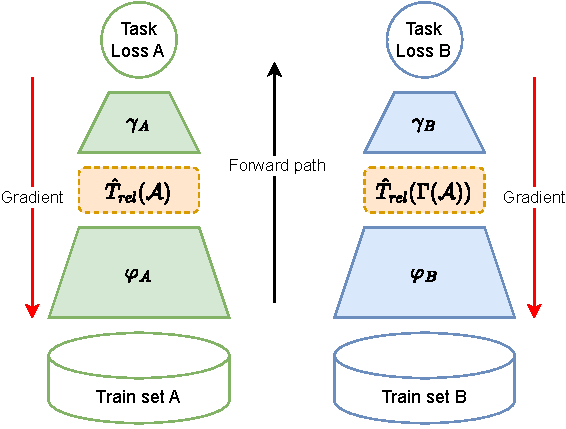
\includegraphics[width=\textwidth]{figures/mt/relativeFullTrainScheme.pdf}
        \caption{Train w/ relative transformations.}
         \label{fig:relFullTrainScheme}
     \end{subfigure}\hfill
      \begin{subfigure}[b]{0.45\textwidth}
         \centering
         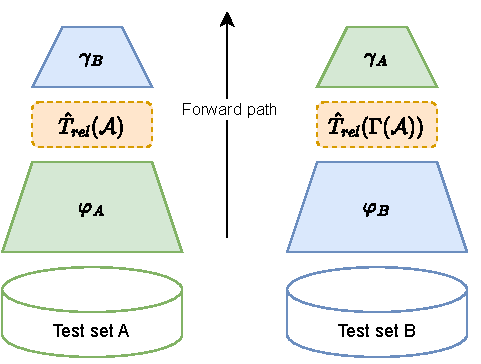
\includegraphics[width=0.9\textwidth]{figures/mt/relativeFullStitchScheme.pdf}
        \caption{Model stitching}
         \label{fig:relFullStitchScheme}
     \end{subfigure}
    \caption{New cross-domain model stitching training and testing}
    \label{fig:fullCrossDomainScheme}
\end{figure}

To be more precise, we will conduct an ablation study based on the experiment presented in \cite{moschella_relative_2022} focusing on multi-lingual Amazon review classification. Due to time constraints, we will focus on cross-lingual stitching, leaving cross-architecture stitching as future work. As the method has been reported to be robust to anchor selection, we will utilize the ``translated'' modality for parallel anchors. In this modality, we first select a number of anchors from the English dataset equal to the dimensionality of the latent space (768 dimensions) and then translate them to other languages using the Google Translator API.\\

However, upon inspecting the provided code from the original relative representation project, we decided to modify the training procedure and the network architecture. This choice is motivated by the identification of several issues and potential methodological concerns:

\begin{itemize}
\item \textit{(bug)} In the case of the 5-class dataset, the code utilized only four classes during both training and testing, despite the network output being five-dimensional. Consequently, a fair assessment of the training performance on the original dataset was not obtained.

\item \textit{(methodological)} When loading the Spanish model, the code failed to restore the dropout probability. This inconsistency in the regularization between the Spanish and other models could arise if the intention is not to freeze the encoder.

\item \textit{(methodological)} The standard Transformer library suggests adding a pooler layer to the classification head while disregarding the one provided in the pretrain model. However, the original code left the pooler layer in the encoder frozen.

\item \textit{(methodological)} An $L^2$ normalization is applied after the relative transformation. The author's rationale for this step was that it improved result robustness. However, we believe that this normalization hinders the analysis of the ablation study of the transformation.

\item \textit{(methodological)} The classification head used SiLU activation and a modified version of InstanceNorm that acted as BatchNorm. Once again, the authors claimed that this architecture was selected based on empirical results. Nevertheless, we suggest employing a more ``standard'' classification head to ensure that the claimed results can be achieved without relying on these less commonly used architectural components.
\end{itemize}


Hence, the proposed new methodology is:
\begin{itemize}
    \item \textbf{Data:}  We will retain the same dataset as the original paper, which involves randomly subsampling 25\% of the Amazon Reviews dataset \cite{keung_multilingual_2020}. As mentioned earlier, we will use the ``translated'' setup to construct the parallel anchors. Training will be conducted on both the coarse-grained version (predicting whether a review is greater or smaller than 3 stars) and the fine-grained version (predicting ratings from 1 to 5 stars).
    
  
    
    \item \textbf{Architecture:} As in the original paper, we will use as encoders the following RoBERTa \cite{liu_roberta_2019} models: ``\texttt{roberta-base}'' for English, ``\texttt{PlanTL-GOB-ES/roberta-base-bne}'' for Spanish, and ``\texttt{ClassCat/roberta-base-french}'' for French. Also, the pooler layer will be removed, and the dropout probability will be initialized to 0.1.
    \begin{lstlisting}[label=code_enc, caption=Decoder Pytorch class]
pooler = nn.Sequential(
            nn.Linear(hidden_size, hidden_size),
            nn.Tanh(),
            nn.Dropout(hidden_dropout_prob)
        )
        
decoder = nn.Sequential(
            nn.Linear(hidden_size, hidden_size),
            nn.GELU(),
            nn.Dropout(hidden_dropout_prob),
            nn.Linear(hidden_size, hidden_size),
            nn.GELU(),
            nn.Dropout(hidden_dropout_prob),
            nn.Linear(hidden_size, num_labels)
        )
    \end{lstlisting}
    The architecture used for the classification head can be seen in Listing~\ref{code_enc}. The number of linear layers remains the same as in the original code, and the standard RoBERTa pooler layer from the Transformer repository is utilized. Additionally, we will employ the same dropout probability as used for the encoder.

    Lastly, as shown in Figure~\ref{fig:fullCrossDomainScheme}, we will use the new \emph{robust relative transformation} developed in the previous section.

    \item \textbf{Training:} Since we want to compare the performance between the fully fine-tuned model against the frozen encoder version, we will have two training setups. For the fully fine-tuned case, we will use layer-wise learning rate decay on the encoder parameters with an initial learning rate of $1.75\cdot 10^{-4}/(num\_labels)$ and decay rate of 0.65. The reason is that we will want to apply the topological regularization in the subsequent experiments, and for this type of loss, we do not need to have significant changes in the initial layers.
    
    The classification head parameters will have an initial learning rate of $10^{-3}/(num\_labels)$ for both setups. Furthermore, we will use an AdamW optimizer with weight decay 0.01, along with the ``\texttt{constant\_schedule\_with\_warmup}'' scheme, incorporating a warmup phase that spans 10\% of the first epoch\footnote{These optimization strategies are considered standard practice when fine-tuning large Transformer models \cite{chang_advanced_2021}.}. We will train the networks for five epochs in the fine-grained and three in the coarse-grained cases.\\


    Due to the size of the transformer models and the reviews, using large batch sizes will exceed the available VRAM. Therefore, we will address this issue using a common technique called gradient accumulation. This involves using a batch size of 16 but updating the network gradients only every $num\_labels$ steps. The corresponding gradients are accumulated during these steps, effectively simulating a batch size of $num\_labels \times 16$. 

    Lastly, for the relative case, we will update the anchor embeddings every $100 \times num\_labels$ steps. This optimization reduces computational costs since the image of 768 samples does not need to be computed at every step. Furthermore, given the employment of layer-wise learning rate decay, we do not anticipate rapid changes in the encoder. Therefore, recomputing the anchor embeddings at every step is unnecessary\footnote{Similar to DQN in RL \cite{mnih_playing_2013} where we periodically freeze the target network, fixing the anchors' embedding every few steps can help stabilize the training. This is because a slight change in the anchor's image could result in critical differences in the geometry of the post-relative latent space.}.

    
    \item \textbf{Testing:} We will evaluate the performance of the stitching in both the absolute (no relative transformation during training) as well as the relative (using the relative transformation) cases. Therefore, as shown in Figure~\ref{fig:relFullStitchScheme}, we will match the encoder language with the one used for the testing dataset, while the decoder can come from any language-specific trained network.
    
    Following the original paper, we will use \glsxtrfull{MAE}, FScore, and \glsxtrfull{ACC} as our metrics. 
    
\end{itemize}

\subsubsection*{Topological regularization analysis}

As we have seen in Section~\ref{sec:topoML}, the original topological regularization paper proposes the following batch construction: We construct each mini-batch, $\mathcal{B}$, as a collection of n sub-batches, i.e., $\mathcal{B} = (\mathcal{B}_1, . . . , \mathcal{B}_b)$. Each sub-batch consists of $n$ samples from the same class, so we end up having an effective batch size of $b\cdot n$.

\begin{figure}[!ht]
    \centering
    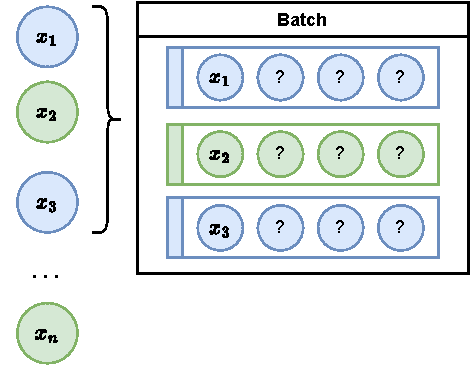
\includegraphics[width=0.5\textwidth]{figures/mt/hoferData.pdf} 
    \caption{Hofer et al.'s original dataloader used for the topological regularization with $b=3$ and $n=4$.}
    \label{fig:hoferData}
\end{figure}


However, when we analyzed the actual implementation, we observed that the batch construction was done as depicted in Figure~\ref{fig:hoferData}:
\begin{enumerate}
    \item We generate $b$-sized samples with random shuffling over the original dataset.
    \item For each point $x_i$ in the batch, we expand the sub-batches by sampling with replacement $n-1$ elements of the same class as $x_i$. 
\end{enumerate}  


We identified two major methodological issues with the utilized dataloader. Firstly, in the presence of significant class imbalances, there is a risk of catastrophic forgetting, as prolonged training steps may occur without encountering the less-represented class. Secondly, this method is computationally intensive since training requires processing the original dataset $n$ times in a single epoch.\\


\begin{figure}[!ht]
    \centering
    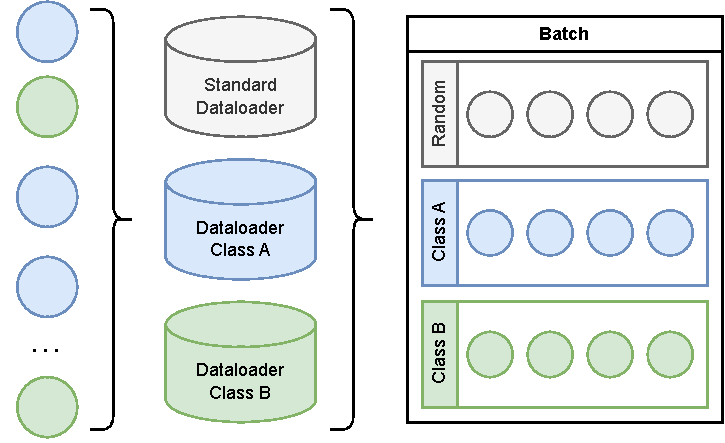
\includegraphics[width=0.7\textwidth]{figures/mt/hoferDataFix.pdf} 
    \caption{New dataloader used for the topological regularization with $b=3$ and $n=4$.}
    \label{fig:hoferDataFix}
\end{figure}


To address these concerns, we propose a new dataloader that follows the high-level description in the original paper while potentially mitigating the aforementioned issues. Figure~\ref{fig:hoferDataFix} illustrates the construction of the new dataloader:
\begin{enumerate}
    \item For each class, we create a separate dataloader containing all samples from that class. Additionally, we create a standard dataloader containing all the samples. These dataloaders utilize shuffling and have a batch size of $n$.
    
    \item We aggregate one batch from each dataloader, resulting in a mini-batch consisting of $num\_classes + 1$ sub-batches. In the case of significant class imbalances, we can iterate through the less-represented class dataloaders until all batches from the most-represented class dataloader have been processed.
    
\end{enumerate}

This new dataloader preserves the sub-class structure necessary for correctly applying the topological regularization loss. Furthermore, its computational overhead is comparable to training directly with the standard dataloader. However, we acknowledge that this new dataloader may potentially encourage the overfitting of the less-represented classes in the presence of significant class imbalances. To counteract this, data augmentation techniques should be employed as a preventive measure. Nonetheless, as depicted in Figure~\ref{fig:clsImb}, our datasets exhibit minimal class imbalances, thus minimizing concerns in this regard.

\begin{figure}[!ht]
    \centering
    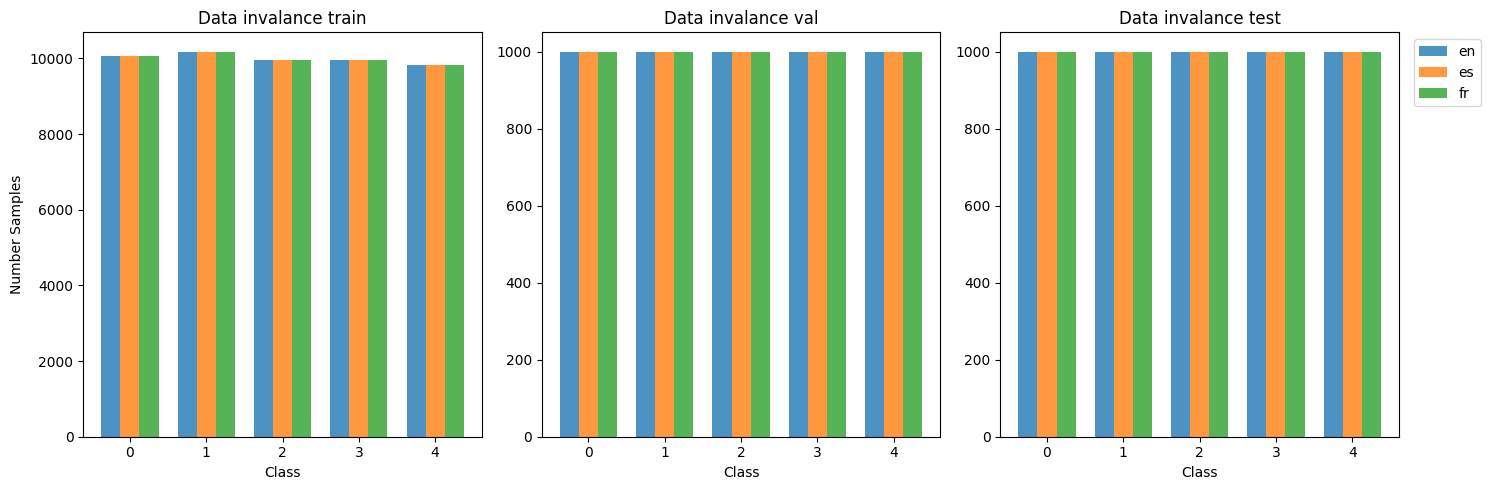
\includegraphics[width=\textwidth]{figures/mt/class_invalance.png} 
    \caption{Class imbalance analysis of the fine-grained datasets w/ 25\% subsampling on the training set.}
    \label{fig:clsImb}
\end{figure}


In Figure~\ref{fig:hoferDataFix}, we introduce an additional random sub-batch in each mini-batch. This extra sub-batch serves as a solution to address an issue encountered when using gradient accumulation with the ``biased'' dataloaders proposed in the original paper. 

Although we previously stated that gradient accumulation should simulate passing the entire mini-batch at once, this assumption only holds true when network components' performance does not depend on the ``input quality''. In our case, we observed that the mean and variance standardization of the robust relative transformation becomes biased with the new dataloader when using gradient accumulation, as we only pass elements from the same class. This issue was not identified in the original paper since the models used were significantly smaller than the RoBERTa models we employ, allowing them to pass the entire mini-batch in each step (without gradient accumulation).

To resolve this problem, we will take the following steps:
\begin{enumerate}
    \item Freeze the parameters of the Linear and LayerNorm modules in the model and set BatchNorm1d and LayerNorm to training mode.
    
    \item Perform a forward pass of the ``random'' mini-batch and compute the cross-entropy loss.
    
    \item Unfreeze the parameters of the Linear and LayerNorm modules in the model and set BatchNorm1d and LayerNorm to eval mode.
    
    \item Pass the remaining $num\_classes$ mini-batches and compute the cross-entropy loss and the topological regularization.

\end{enumerate}
By adopting this approach, we can utilize the running averages of the mean and variance computed on unbiased sub-batches during the forward pass of the biased sub-batches.\\

In our ablation studies, we will utilize a classification head consisting of only one linear layer without even including a pooling layer. While there is no theoretical constraint on the classification head for applying topological regularization, we have two primary methodological justifications for this choice.

Firstly, we could see a more expressive classification head as an implicit regularization scheme. By using a simpler decoder, we intentionally reduce variance and increase bias, allowing the model to overfit the training data. This setup requires the aid of explicit regularization techniques, such as topological densification, to reduce the generalization error.

Secondly, the objective of the topological regularization loss is to encourage a more favorable configuration of the latent space for the classification task. However, if we employ a complex classification head, we may not require the assistance of these losses, as the model could potentially fit more intricate decision boundaries.

It is important to note that this setup is not unrealistic, as popular Transformer networks like Vision Transformers (ViTs) \cite{dosovitskiy_vit_2021} often employ one or two linear layers (depending on the specific implementation) for their classification heads.\\


Figure~\ref{fig:topoSetups} presents the different topological regularization setups we will explore when using the relative transformation. Firstly, we will analyze the case of applying topological regularization both before (pre-relative) and after (post-relative) the relative transformation. Additionally, based on empirical results discussed in Chapter~\ref{ch:resultsAndAnalysis}, we will also apply $L^2$ topological regularization using the same $\beta$ hyperparameter both before and after the relative transformation simultaneously.



\begin{figure}[ht!]
     \centering
    \begin{subfigure}[b]{0.45\textwidth}
         \centering
         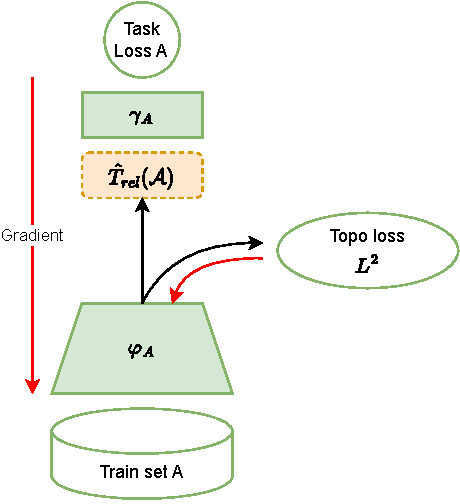
\includegraphics[width=0.9\textwidth]{figures/mt/relativeTopoPreScheme.pdf}
        \caption{Pre-relative}
         \label{fig:relativeTopoPreScheme}
         \vspace*{3mm}
     \end{subfigure}
     \hfill
      \begin{subfigure}[b]{0.45\textwidth}
         \centering
         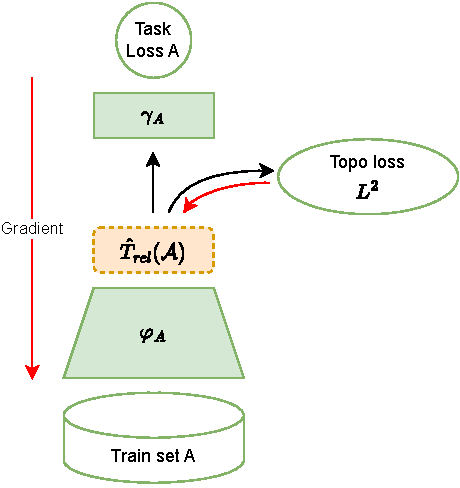
\includegraphics[width=0.9\textwidth]{figures/mt/relativeTopoPostScheme.pdf}
        \caption{Post-relative}
         \label{fig:relativeTopoPostScheme}
         \vspace*{3mm}
     \end{subfigure}
      \vspace{\fill}
       \begin{subfigure}[b]{0.45\textwidth}
         \centering
         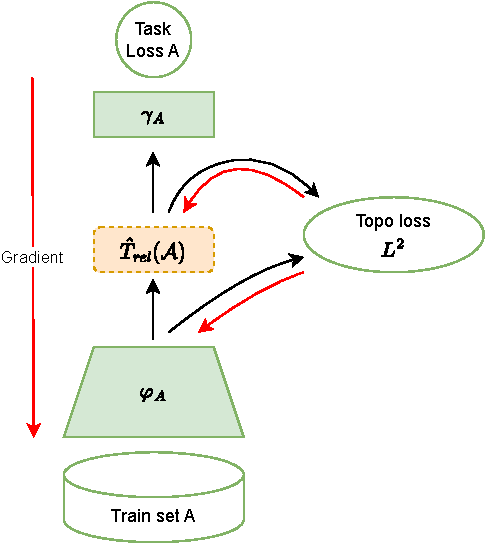
\includegraphics[width=0.9\textwidth]{figures/mt/relativeTopoBothScheme.pdf}
        \caption{Both $L^2$}
         \label{fig:relativeTopoBothScheme}
     \end{subfigure}
      \hfill
      \begin{subfigure}[b]{0.45\textwidth}
         \centering
         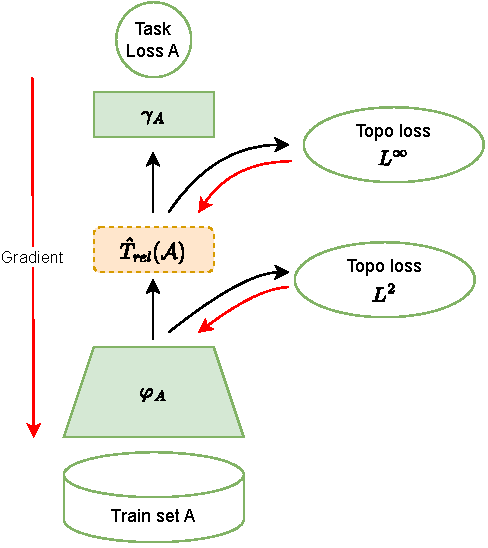
\includegraphics[width=0.9\textwidth]{figures/mt/relativeTopoMixScheme.pdf}
        \caption{Mix $L^2$ and $L^\infty$}
         \label{fig:relativeTopoMixScheme}
     \end{subfigure}
    \caption{Different topological regularization setups while using relative transformation.}
    \label{fig:topoSetups}
\end{figure}


Lastly, as shown in Figure~\ref{fig:relativeTopoMixScheme}, we also use the $L^\infty$ metric to construct the Vietorus Rips filtration used for the post-relative topological regularization. There are two methodological justifications for using this metric:
\begin{enumerate}
    \item TDA methods analyze and utilize the topological features of the underlying data manifold. However, they are also geometric methods, and better results can be achieved by employing a distance metric that aligns with the geometry of the data manifold. Since the relative transformation codomain is $[-1, 1]^k$, where $k$ is the number of anchors, $L^\infty$ open balls are a better fit than $L^2$ balls.

    \item Determining the optimal value of the $\beta$ hyperparameter in a high-dimensional latent space can be challenging, even though we understand its meaning. In the original paper, the best $\beta$ value was obtained through extensive hyperparameter tuning.

    To provide an intuition for selecting $\beta$, we developed a new heuristic based on the empirical distribution of the 0-homology death times and the maximum death times of the test set\footnote{This plots might reassemble the persistence images presented in Section~\ref{sec:topoML}. However, in this case, we do not have a 2D image because by using $\text{H}_0(\text{VR})$, all the points lie in the line $x=0$. Furthermore, instead of a heat map, we plot the density estimation.}, as depicted in Figure~\ref{fig:h0Ex}. With this understanding of the topology without any imposed regularization, we can make more informed choices for different $\beta$ values rather than relying on random selection.

    \begin{figure}[!ht]
        \centering
        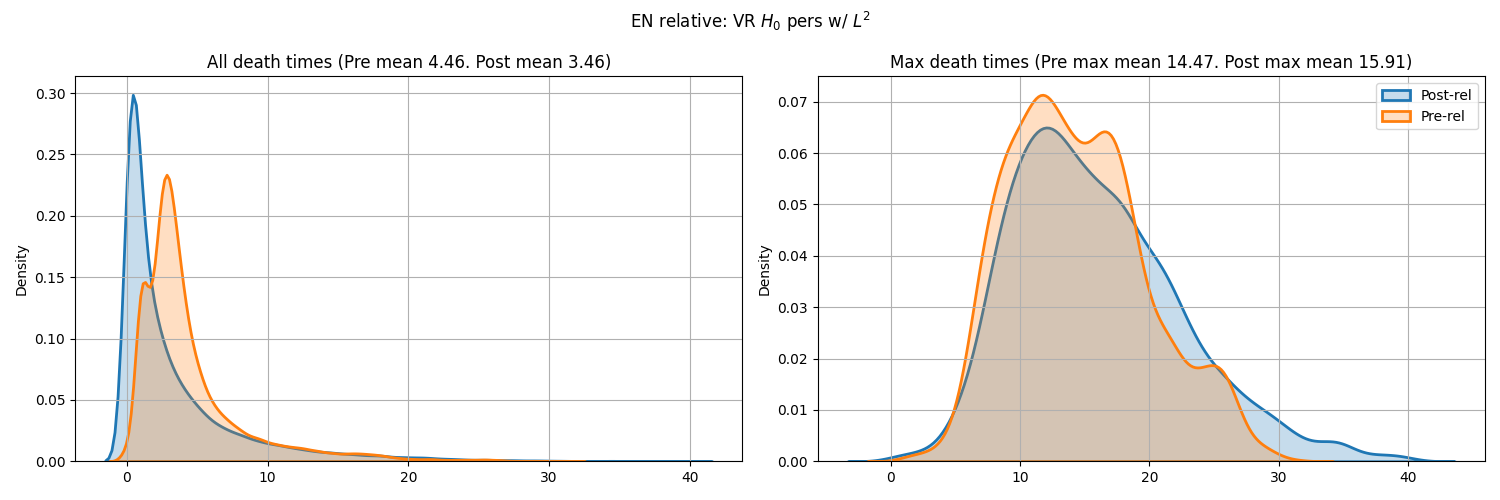
\includegraphics[width=\textwidth]{figures/mt/en_relative_seed0.png} 
        \caption{Example of the death time distributions.}
        \label{fig:h0Ex}
    \end{figure}

   Nevertheless, using the $L^\infty$ metric allows for a more concise interpretation of this hyperparameter. In an optimal scenario where each cluster has only one anchor at its centroid, the maximum coordinate of the relative transformation corresponds to the cosine of the angle between a point and the center of its cluster. Therefore, we can argue that the $\beta$ hyperparameter, when using $L^\infty$, relates to the optimal spread of the cluster in terms of angle, given by $\beta = 1 - \cos(\pi\theta/180)$.
\end{enumerate}


Lastly, we want to remark that due to time constraints, we will focus this analysis on a random 1\% sub-sample of the fine-grained dataset. Furthermore, we will train our networks for 40 epochs to ensure that the topological regularization prevents overfitting. We will also use a ``\texttt{cosine\_schedule\_with\_warmup}'' scheduler on the learning rate and a linear cyclic scheduler for the weight $\lambda$ component of the regularization loss. This cyclic scheduler has been previously used in VAEs to obtain a better synergy between the classification loss and the regularization \cite{fu_cyclical_2019}.


\end{document}
